\section{The Symmetric Group}

We have seen various examples of groups containing numbers, matrices, and sets. Stranger still is the group called the Symmetric, or permutation, group. This particular group contains all the functions over a set up to permutation (hence the name).

\begin{definition}{Symmetric Group}
	Let $X$ be a set. The symmetric group on $X$, denoted $Sym_{X}$ or $S_{X}$, is the group of all bijections on $X$ under the operation of function composition, $\circ$.
\end{definition}

The typical notation we will see is $Sym_{n}$, where $n$ is indicative of the set $\{1,2,3,\dots,n\}$; hence, when we take $\sigma\in Sym_{n}$, we know $\sigma:\{1,2,\dots,n\}\mapsto\{1,2,\dots,n\}$ where $\sigma$ is a bijection.

\begin{example}{Determine $\sigma(x)\ \forall x\in\{1,2,3,4,5\}$ given}
	{\egft{
		\[
			\left[
			\begin{array}{c c c c c}
				1 & 2 & 3 & 4 & 5 \\
				3 & 1 & 2 & 5 & 4
			\end{array}
			\right]
		\]
	}}
	The notation here can be confusing at first; it reads from top to bottom saying that the top element gets mapped to the element below it. Hence
	\[
		\sigma(1)=3,\qquad \sigma(2) = 1,\qquad \sigma(3)=2,\qquad \sigma(4)=5,\qquad\sigma(5)=4.
	\]
\end{example}
Luckily, we have another way to write the permutation given by the matrix in the previous example. It is called cycle notation, an it describes the mappings that are made by a particular function.

\subsection*{Cycles}
Let's begin with an example showing how to write a matrix in cycle notation.

\begin{example}{Write the following in cycle notation.}
	{\egft{
		\[
			\left[
			\begin{array}{c c c c c}
				1 & 2 & 3 & 4 & 5 \\
				3 & 1 & 2 & 5 & 4
			\end{array}
			\right]
		\]
	}}
	Again, we read this matrix from top to bottom to determine where elements get sent. Starting with 1, we see
	\[
		1\mapsto3\mapsto2\mapsto1.
	\]
	We write the corresponding cycle as
	\[
		(1\ 3\ 2).
	\]
	This doesn't cover every element, however, so we start with 4 and see
	\[
		4\mapsto5\mapsto4\implies(4\ 5).
	\]
	Hence, $\sigma$ is given by the product of the two cycles.
	\[
		(1\ 3\ 2)(4\ 5).
	\]
\end{example}
Every cycle within a permutation can be represented as it's own permutation within $Sym_{n}$. In other words, we represent each cycle as it's own function, typically called $\gamma$, where $\gamma_{i}$ and $\gamma_{j}$ are disjoint from each other. The function $\gamma$ is called a $k$-cycle.
\begin{definition}{$k$-cycle}
	A $k$-cycle in $Sym_{n}$ is a permutation $\gamma$ such that given the cycle $(x_{1}\ x_{2}\ \dots\ x_{k})$,
	\begin{enumerate}
		\item
		      \[
		      	\gamma(x_{i})=
		      	\begin{cases}
		      		x_{i+1}\qquad\text{if }i\neq k \\
		      		x_{1}\qquad\text{if }i = k
		      	\end{cases},
		      \]
		      and
		\item if $y\neq x_{i}\ \forall i\in(0,k]$, then $\gamma(y)=y$.
	\end{enumerate}
    If $\gamma$ is a 2-cycle, then we call $\gamma$ a transposition.
\end{definition}
All this definition is saying is that if an element is in the cycle then we go to next element in the cycle, and if we have an element not in the cycle, we fix it.

\begin{example}{Conisder the cycle $\gamma=(1\ 984\ 21212\ 189\ 493\ 2278\ 1999)\in Sym_{1000000}$. Determine}
	{\egft{\begin{enumerate}
			\item $\gamma(21212)$
			\item $\gamma(1999)$
			\item $\gamma(13579)$
		\end{enumerate}}}
    We know that $\gamma$ is a 7-cycle, so we can use the definition of $k$-cycle to figure out the answers. Since 21212 is in the cycle, we just move to the next element in the cycle. Hence
    \[
        \gamma(21212)=189.
    \]
    Similarly, 1999 is in the cycle, but we must return back to the front of the cycle according to the definition.
    \[
        \gamma(1999)=1.
    \]
    Finally, 13579 is not in the cycle, so we have
    \[
        \gamma(13579)=13579.
    \]
\end{example}

One of the reasons that we like cycles so much is that we can decompose any permutation into a product of disjoint cycles, much like factoring a number, and that decomposition will be unique up to order. Out of this comes our first major theorem about symmetric groups.

\begin{theorem}{}
    Let $\sigma\in Sym_{n}$. Then there exist disjoint cycles $\gamma_{1},\gamma_{2},\dots,\gamma_{n}$ such that
    \begin{enumerate}
        \item $\sigma=\gamma_{1}\gamma_{2}\dots\gamma_{n}$
        \item The decomposition is unique up to order.
    \end{enumerate}
\end{theorem}
\begin{proof}
    Take $\sigma\in Sym_{n}$ and let $x_{1}$ be the minimal element in $\{1,2,\dots,n\}$ such that $\sigma(x_{1})\neq x_{1}$. Then we can write
    \begin{gather*}
        \sigma(x_{1})=x_{2}\\
        \sigma(x_{2})=x_{3}\\
        \vdots
    \end{gather*}
    Since there are finitely many $x_{i}$, we will eventually repeat one of these statements. Thus, there will be a minimal $m$ where $\sigma(x_{m})=x_{i}$ and $\sigma(x_{i-1})=x_{i}$, so $x_{m}=x_{i-1}$ since $\sigma$ is bijective.
    We chose $m$ to be minimal, so it follows that $x_{i}=x_{1}$. Then $\sigma=\gamma_{1}\sigma'$ where
    $\gamma_{1}=(x_{1}\ x_{2}\ \dots\ x_{m})$ and $\sigma'$ is disjoint from $\gamma_{1}$. Repeating the process for $\sigma=\sigma'$ will yield the result. The proof of uniqueness is tedious, so we will not do it here.
\end{proof}

The proof of this theorem is very worthwhile to go through since it outlines how to find $\gamma_{i}$.

The next topic we will to cover in regards to cycles is how to multiply cycles. Recall that the operation on $Sym_{n}$ is function composition; as such, multiplying cycles is the same as composing the functions that they represent.
\begin{example}{Given $\sigma=(1\ 2\ 3)(3\ 4\ 5)$ and $\tau=(4\ 2\ 3\ 5)$, find $\sigma\tau$.}
    We are looking for the result of $(1\ 2\ 3)(3\ 4\ 5)(4\ 2\ 3\ 5)=\gamma_{1}\gamma_{2}\gamma_{3}$. To find out what happens to 1, we need
    \begin{align*}
        \gamma_{1}(\gamma_{2}(\gamma_{3}(1))) &= \gamma_{1}(\gamma_{2}(1))\\
        &= \gamma_{1}(1)\\
        &= 2.
    \end{align*}
    Hence, $1\mapsto2$. Now we trace 2 through the functions, and so on. We will find that
    \[
        (1\ 2\ 3)(3\ 4\ 5)(4\ 2\ 3\ 5)=(1\ 2\ 4\ 3)(5).
    \]
    We usually don't write 1-cycles, so the solution is $(1\ 2\ 4\ 3)$.
\end{example}

\subsection*{Properties of $Sym_{n}$}

Since $Sym_{n}$ is a group, we know that it must contain an identity element. We don't call the identity function $e$, but rather $id$, and it is given by $id(n)=n\ \forall n\in X_{n}$. We also know that $Sym_{n}$ will contain inverse elements for each $\sigma\in Sym_{n}$, but we must discuss some more properties of $Sym_{n}$ before looking at inverses.

Another property we would like to know is whether or not elements of the symmetric group commute, and if not, when do they commute. In general, $Sym_{n}$ is \textbf{not} abelian. Consider $Sym_{6}$.
\begin{example}{Show that $Sym_{3}$ is not abelian}
	We must only find one counterexample in order to show that it is not abelian. Let
	\[
		\sigma=(2\ 3),\qquad\tau=(1\ 2\ 3).
	\]
	Then $\sigma\tau=(1\ 3)$, but $\tau\sigma=(1\ 2)$, so $Sym_{6}$ is not abelian.
\end{example}
The only case in which $Sym_{n}$ is abelian is when $n=2$, since there are only 2 elements in $Sym_{2}$. We know this since
\begin{theorem}{}
    The order of $Sym_{n}$ is $n!$.
\end{theorem}
\begin{proof}
    This is not something worth proving. It relies on ideas from combinatorics.
\end{proof}

Since $Sym_{n}$ is so large for $n\geq5$, we tend to stick with small $n$. We know that $Sym_{n}$ is not abelian generally, but there are cases in which its elements commute. Given permutations $\gamma_{1},\gamma_{2},\dots,\gamma_{n}$, the composition will commute provided that all the permutations are disjoint.
It follows then that
\[
    (\gamma_{1},\gamma_{2},\dots,\gamma_{n})^{k}=\gamma_{1}^{k},\gamma_{2}^{k},\dots,\gamma_{n}^{k}.
\]
This leads us to our next theorem.
\begin{theorem}{}
    If $\sigma$ is the composition of $m$ disjoint permutations $\gamma_{i}$, then
    \[
        |\sigma|= \lcm(|\gamma_{1}|,|\gamma_{2}|,\dots,|\gamma_{m}|).
    \]
\end{theorem}
\begin{proof}
    Since the permutations are disjoint, we have that
    \[
        \sigma^{k}=\gamma_{1}^{k}\gamma_{2}^{k}\dots\gamma_{m}^{k}.
    \]
    If $k=|\sigma|$, then $ord(\gamma_{i})\mid k\ \forall i$. The order of an element is the least such positive integer such that $\gamma^{n}=id$, so it follows that $|\sigma|=\lcm(|\gamma_{1}|,|\gamma_{2}|,\dots,|\gamma_{m}|)$ Since the least common multiple is the least such.
\end{proof}
We now have a manner in which to calculate the order of any permutation in $Sym_{n}$, analogous to the way we can calculate the order of any element in $\ZZ_{n}$. We originally wanted to discuss the inverses of elements in $Sym_{n}$; it turns out we have a way of forming inverses with relative ease.
\begin{theorem}{}
    Let $\gamma=(x_{1}\ x_{2}\ \dots\ x_{k})$. Then $\gamma^{-1}=(x_{1}\ x_{k}\ x_{k-1}\ \dots\ x_{3}\ x_{2})$.
\end{theorem}
\begin{proof}
    Define $\tau=(x_{1}\ x_{k}\ x_{k-1}\ \dots\ x_{3}\ x_{2})$. Then
    \begin{gather*}
        \tau\gamma(x_{i})=\tau(x_{i+1})=x_{i}\\
        \tau\gamma(x_{k})=\tau(x_{1})=x_{k}.
    \end{gather*}
\end{proof}
There's a nice corollary to this theorem.
\begin{corollary}
    Let $\sigma=\gamma_{1}\gamma_{2}\dots\gamma_{n}$ where each $\gamma$ is disjoint. Then
    \[
        \sigma^{-1}=\gamma_{1}^{-1}\gamma_{2}^{-1}\dots\gamma_{n}^{-1}.
    \]
\end{corollary}

All of the theorems we have seen thus far have dealt with disjoint cycles, but what happens when we have non-disjoint cycles? As it happens, we can simply compose the cycles which will always give us disjoint cycles. We also have the power to go the other way; if $\sigma$ is given to us as disjoint cycles, we can write it as a series of transpositions. This is useful to us when we want to know the sign of the permutation.

\begin{definition}{Sign of a Permutation}
    Let $\sigma$ be a permutation. Then the sign of $\sigma$ is given by
    \[
        sgn(\sigma)=
        \begin{cases}
            1 \qquad\ \ \text{ if }\sigma\text{ is composed of an even number of transpositions}\\
            -1 \qquad \text{ if }\sigma\text{ is composed of an odd number of transpositions}\\
        \end{cases}.
    \]
\end{definition}
If we have a $k$-cycle $\gamma$, then it follows that $sgn(\gamma)=(-1)^{k-1}$. The sign function leads us to a very important subgroup of $Sym_{n}$.

\subsection*{The Alternating Group}
The sign of permutations is of great concern to us since the set of even permutations in $Sym_{n}$ form a group called the alternating group.

\begin{definition}{The Alternating Group}
    The alternating group, $Alt_{n}$, is the subgroup of $Sym_{n}$ given by
    \[
        Alt_{n}=\{\sigma\in Sym_{n}: sgn(\sigma)=1\}.
    \]
\end{definition}
We should probably show that it is indeed a subgroup.
\begin{example}{Show $Alt_{n}\leq Sym_{n}$}
    The identity is in $Alt_{n}$ since it consists of 0 transpositions. Closure follows almost immediately; inverses are also immediate since $|\sigma|=|\sigma^{-1}|$.
\end{example}

We may also be interested in the order of the alternating group. $Sym_{n}$ has order $n!$ since it consists of all permutations of bijective functions. It turns out that the alternating group consists of half of these permutations.
\begin{theorem}{}
\[
	|Alt_{n}|= \frac{n!}{2}.
\]
\end{theorem}
\begin{proof}
	Let $Odd_{n}$ be the set of all odd permutations on $n$. Then $Alt_{n}\cup Odd_{n}=Sym_{n}$, and $Alt_{n}\cap Odd_{n}=\emptyset$. If we can create a bijection $f:Alt_{n}\to Odd_{n}$, then we are done.
	Define $f(\sigma)=(1\ 2)\sigma$. The function $f$ is invertible since
	\[
		f(\sigma_{1})=f(\sigma_{2})\implies
		(1\ 2)\sigma_{1}=(1\ 2)\sigma_{2}\implies
		\sigma_{1}=\sigma_{2}.
	\]
	To see that $f$ is surjective, let $\psi$ be an odd permutation. Then $f((1\ 2)\psi)=(1\ 2)(1\ 2)\psi=\psi$.
\end{proof}

This proof gives us insight to an odd occurrence within $Sym_{n}$; $Alt_{n}\leq Sym_{n}$, but $Odd_{n}\not\leq Sym_{n}$.
One reason that $Odd_{n}$ is not a subgroup of $Sym_{n}$ is its lack of identity function, since $id$ is an even permutation. There is an interesting corollary to this proof that gives us more information about the subgroups of $Sym_{n}$.

\begin{corollary}
	Let $H\leq Sym_{n}$. Then $H\leq Alt_{n}$ or $H$ consists of exactly half even and half odd permutations.
\end{corollary}
\begin{proof}
	Assume $H\not\leq Alt_{n}$. Let $H_{o}$ be the odd permutations and $H_{e}$ be the even permutations. Then
	\[
		H = H_{o} \coprod H_{e}.
	\]
 	Since the union is disjoint, we simply need to show that there is a bijective function from $H_{o}$ to $H_{e}$. Let $\tau\in H_{o}$, and define $f:H_{e}\to H_{o}$ by $f(\sigma)=\tau\sigma$. We leave it to you to show this is a bijective function.
\end{proof}

\subsection*{The Dihedral Group}

The dihedral group on $n$ objects, $D_{n}$ or $Dih_{n}$, is a subgroup of the symmetric group that describes the geometric transforms we can perform on an $n$-gon. We will discuss $Dih_{4}$ here in depth, but $Dih_{n}\leq Sym_{n}\ \forall n$. Consider the following square with its labeled corners.
\begin{center}
	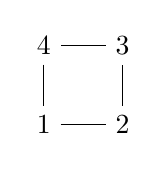
\begin{tikzpicture}[node distance=1cm]
		\node(1) {1};
		\node(2) [right of=1] {2};
		\node(3) [above of=2] {3};
		\node(4) [above of=1] {4};

		\draw(1) -- (2);
		\draw(2) -- (3);
		\draw(3) -- (4);
		\draw(4) -- (1);
	\end{tikzpicture}
\end{center}
The permutations within $Dih_{4}$ represent the mappings of the four corners. Consider simple rotations of the square given by the function $\rho$; $\rho(n)$ will represent a rotation by $\pi/2$. We typically in the math world consider counterclockwise to be the positive direction.
\begin{center}
	\begin{tabular}{c c c c}
		Rotation by $\pi/2$ & Rotation by $\pi$ & Rotation by $3\pi/2$ & Rotation by $2\pi$\\
		\hline
		&&&\\
		$\rho=(1\ 2\ 3\ 4)$ & $\rho^{2}=(1\ 3)(2\ 4)$ & $\rho^{3}=(1\ 4\ 3\ 2)$ & $\rho^{4}=id$\\
		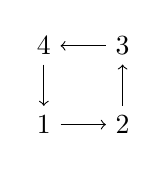
\begin{tikzpicture}[node distance=1cm]
			\node(1) {1};
			\node(2) [right of=1] {2};
			\node(3) [above of=2] {3};
			\node(4) [above of=1] {4};

			\draw[->](1) -- (2);
			\draw[->](2) -- (3);
			\draw[->](3) -- (4);
			\draw[->](4) -- (1);
		\end{tikzpicture} &
		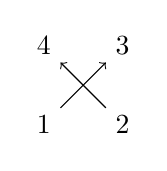
\begin{tikzpicture}[node distance=1cm]
			\node(1) {1};
			\node(2) [right of=1] {2};
			\node(3) [above of=2] {3};
			\node(4) [above of=1] {4};

			\draw[->](1) -- (3);
			\draw[->](2) -- (4);
		\end{tikzpicture} &
		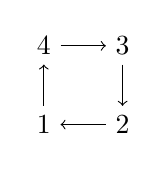
\begin{tikzpicture}[node distance=1cm]
			\node(1) {1};
			\node(2) [right of=1] {2};
			\node(3) [above of=2] {3};
			\node(4) [above of=1] {4};

			\draw[->](1) -- (4);
			\draw[->](2) -- (1);
			\draw[->](3) -- (2);
			\draw[->](4) -- (3);
		\end{tikzpicture}&
		\begin{tikzpicture}[node distance=1cm]
			\node(1) {1};
			\node(2) [right of=1] {2};
			\node(3) [above of=2] {3};
			\node(4) [above of=1] {4};
		\end{tikzpicture}\\
		%
		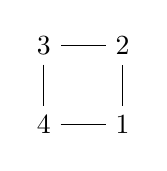
\begin{tikzpicture}[node distance=1cm]
			\node(1) {4};
			\node(2) [right of=1] {1};
			\node(3) [above of=2] {2};
			\node(4) [above of=1] {3};

			\draw(1) -- (2);
			\draw(2) -- (3);
			\draw(3) -- (4);
			\draw(4) -- (1);
		\end{tikzpicture} &
		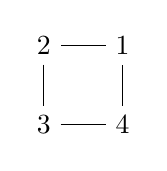
\begin{tikzpicture}[node distance=1cm]
			\node(1) {3};
			\node(2) [right of=1] {4};
			\node(3) [above of=2] {1};
			\node(4) [above of=1] {2};

			\draw(1) -- (2);
			\draw(2) -- (3);
			\draw(3) -- (4);
			\draw(4) -- (1);
		\end{tikzpicture} &
		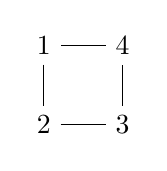
\begin{tikzpicture}[node distance=1cm]
			\node(1) {2};
			\node(2) [right of=1] {3};
			\node(3) [above of=2] {4};
			\node(4) [above of=1] {1};

			\draw(1) -- (2);
			\draw(2) -- (3);
			\draw(3) -- (4);
			\draw(4) -- (1);
		\end{tikzpicture} &
		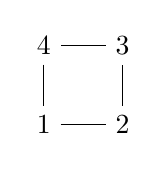
\begin{tikzpicture}[node distance=1cm]
			\node(1) {1};
			\node(2) [right of=1] {2};
			\node(3) [above of=2] {3};
			\node(4) [above of=1] {4};

			\draw(1) -- (2);
			\draw(2) -- (3);
			\draw(3) -- (4);
			\draw(4) -- (1);
		\end{tikzpicture}
	\end{tabular}
\end{center}

The bottom row of squares represents the permutation after $\rho$ has been applied to the original square. Rotation are not the only transformation we can apply to the square, however; we can flip the square across all of its symmetric axes.
\begin{center}
	\begin{tabular}{c c c c}
		Flip over $y$-axis & Flip over $x$-axis & Flip over off diagonal & Flip over main diagonal\\
		\hline
		&&&\\
		$\sigma=(1\ 2)(3\ 4)$ & $\tau=(1\ 4)(2\ 3)$ & $\delta_{1}=(4\ 2)$ & $\delta_{2}=(1\ 3)$\\
		\begin{tikzpicture}[node distance=1cm]
			\node(1) {1};
			\node(2) [right of=1] {2};
			\node(3) [above of=2] {3};
			\node(4) [above of=1] {4};

			\draw[->](1) -- (2);
			\draw[->](3) -- (4);
		\end{tikzpicture} &
		\begin{tikzpicture}[node distance=1cm]
			\node(1) {1};
			\node(2) [right of=1] {2};
			\node(3) [above of=2] {3};
			\node(4) [above of=1] {4};

			\draw[->](1) -- (4);
			\draw[->](2) -- (3);
		\end{tikzpicture} &
		\begin{tikzpicture}[node distance=1cm]
			\node(1) {1};
			\node(2) [right of=1] {2};
			\node(3) [above of=2] {3};
			\node(4) [above of=1] {4};

			\draw[->](4) -- (2);
		\end{tikzpicture} &
		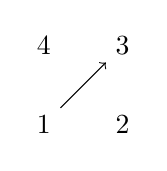
\begin{tikzpicture}[node distance=1cm]
			\node(1) {1};
			\node(2) [right of=1] {2};
			\node(3) [above of=2] {3};
			\node(4) [above of=1] {4};

			\draw[->](1) -- (3);
		\end{tikzpicture}\\
		%TODO put things in here
		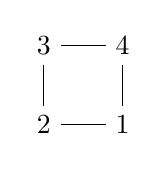
\begin{tikzpicture}[node distance=1cm]
			\node(1) {2};
			\node(2) [right of=1] {1};
			\node(3) [above of=2] {4};
			\node(4) [above of=1] {3};

			\draw(1) -- (2);
			\draw(2) -- (3);
			\draw(3) -- (4);
			\draw(4) -- (1);
		\end{tikzpicture}&
		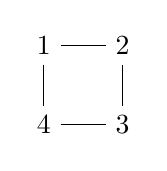
\begin{tikzpicture}[node distance=1cm]
			\node(1) {4};
			\node(2) [right of=1] {3};
			\node(3) [above of=2] {2};
			\node(4) [above of=1] {1};

			\draw(1) -- (2);
			\draw(2) -- (3);
			\draw(3) -- (4);
			\draw(4) -- (1);
		\end{tikzpicture}&
		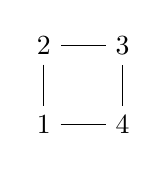
\begin{tikzpicture}[node distance=1cm]
			\node(1) {1};
			\node(2) [right of=1] {4};
			\node(3) [above of=2] {3};
			\node(4) [above of=1] {2};

			\draw(1) -- (2);
			\draw(2) -- (3);
			\draw(3) -- (4);
			\draw(4) -- (1);
		\end{tikzpicture}&
		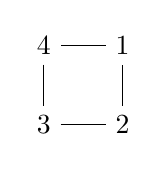
\begin{tikzpicture}[node distance=1cm]
			\node(1) {3};
			\node(2) [right of=1] {2};
			\node(3) [above of=2] {1};
			\node(4) [above of=1] {4};

			\draw(1) -- (2);
			\draw(2) -- (3);
			\draw(3) -- (4);
			\draw(4) -- (1);
		\end{tikzpicture}
	\end{tabular}
\end{center}
These eight rotations are all the possible geometric transforms we can perform on a square; it's no coincidence that this is twice the number of vertices on the $n$-gon. We actually know the order of any $Dih_{n}$.
\begin{theorem}{}
	\[|Dih_{n}|=2n.\]
\end{theorem}
We won't prove this here, but the idea is similar to the proof of the size of $Alt_{n}$.
